\scanpage{164}

\[
\tau',\ \uline{\tau''},\ \uline{\sigma},\ \uline{\rho'},\ \rho''
\qquad \deleted{\unsure{\sigma|\tau}}
\]
\[
\left\{\begin{aligned}
&\tau'^2=\tau''^2=\sigma^4=1\qquad \sigma^2=\tau'\tau'',\quad
 \deleted{\sigma(\rho')=\rho}\\
&\tau'(\rho')=\tau''(\rho')=\rho'^{-1},\qquad
 \unsure{\tau'|\tau''}(\rho'')=\tau''(\rho'')=\rho''^{-1}\\
&\sigma(\rho')=\rho''\qquad(\Rightarrow\sigma(\rho'')=\rho')\\
&(\sigma\rho')^3\unsure{\sim|\simeq}1\quad\text{dans }\mathcal T^+_{1,1}
\end{aligned}\right.
\]
\hfill (mais \inserted{non} dans un groupe spécial)

\diagram{\[
\begin{array}{rcl|l}
\rho'&\longmapsto&\varepsilon_0&\\
\rho''&\mathrel{\mapstochar\! -\! -}&\varepsilon_1&\\[3pt]
\tau''&\longmapsto&\tau_\infty=\tau=r_\infty&\\[3pt]
\tau'&\longmapsto&\omega_0\tau_\infty=-\tau&\\[3pt]
\sigma&\mathrel{\mapstochar\! -\! -}&\sigma_\infty=\sigma&
\end{array}
\]}

\[
\sigma^{-1}\rho'=\sigma^3\rho'\longmapsto
 \sigma^3\varepsilon_0=\sigma^3(\sigma\rho)=\rho
\]
\[
\tau''\sigma\longmapsto\tau'_\infty=r_0
\]
\[
\tau''\rho'=\underbrace{(\tau''\sigma)}_{\mapsto r_0}
 \underbrace{(\sigma^{-1}\rho')}_{\mapsto\rho}
 \mathrel{\mapstochar\! -\! -}r_1
\]

\diagram{\[
\begin{array}{|rcl|rcl|}\hline
\tau''&\longmapsto&r_\infty&\rho'&\mathrel{\mapstochar\! -\! -}&\varepsilon_0\\
\tau''\sigma&\longmapsto&r_0&\sigma&\longmapsto&\sigma\\
\tau''\rho'&\longmapsto&r_1&\sigma^{-1}\rho'&\mathrel{\mapstochar\! -\! -}&\rho\\\hline
\end{array}
\]}
\[
\unsure{\mathfrak X|\mathcal X}=(X,X',X'')
\]

\figure{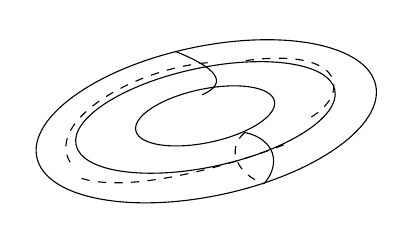
\begin{tikzpicture}[x=1cm,y=1cm,rotate=12]
\draw (0,0) ellipse (2.2 and .95);
\draw (0,.05) ellipse (1.68 and .63);
\draw (0,.07) ellipse (.9 and .34);
\draw[dashed] (-1.8,-.15) .. controls (-2,.45) and (-.7,.85) .. (.2,.72);
\draw[dashed] (.65,.65) .. controls (1.95,.55) and (1.85,-.05) .. (1.3,-.23);
\draw[dashed] (-1.7,-.38) .. controls (-1.1,-.72) and (.35,-.6) .. (1,-.48);
\draw (-.2,.95) .. controls (.25,.65) and (.4,.42) .. (.02,.34);
\draw (.45,-.24) .. controls (.8,-.4) and (.83,-.72) .. (.55,-.93);
\draw[dashed] (.45,-.24) .. controls (.16,-.4) and (.25,-.74) .. (.55,-.93);
\end{tikzpicture}}

\figure{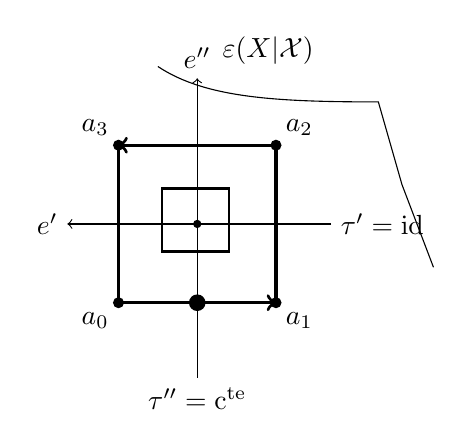
\begin{tikzpicture}[x=1cm,y=1cm]
\draw[very thick] (0,0) rectangle (2,2);
\draw[very thick,->] (0,0)--(2,0);
\draw[very thick,->] (2,2)--(0,2);
\draw[thick] (.55,.65) rectangle (1.4,1.45);
\draw[->] (2.7,1)--(-.65,1) node[left] {$e'$};
\draw[->] (1,-.95)--(1,2.85) node[above] {$e''$};
\fill (0,0) circle (2pt) node[below left] {$a_0$};
\fill (2,0) circle (2pt) node[below right] {$a_1$};
\fill (2,2) circle (2pt) node[above right] {$a_2$};
\fill (0,2) circle (2pt) node[above left] {$a_3$};
\fill (1,0) circle (3pt);\fill (1,1) circle (1.5pt);
\node[right] at (2.7,1) {$\tau'=\mathrm{id}$};
\node[below] at (1,-.95) {$\tau''=\mathrm{c}^{\mathrm{te}}$};
\node at (1.9,3.2) {$\varepsilon(\unsure{\mathfrak X|\mathcal X})$};
\draw (.5,3) .. controls (1.1,2.6) and (2,2.55) .. (3.3,2.55)
 --(3.6,1.5)--(4,.45);
\end{tikzpicture}}

$\{X',X''\}={}$ ens des codiagonales du carré

$\varepsilon_0(X')\simeq{}$ ens des deux côtés opposés du carré qui correspondent à \unsure{le|la} $X''$

$\varepsilon_1(X')\simeq{}$ ens des deux côtés opposés du carré qui correspondent à $X'$

\margin{$\varepsilon(\unsure{\mathfrak X|\mathcal X})\ \deleted{\unsure{\varepsilon_0(X')|\varepsilon_1(X')}}$}
\margin{\deleted{\unsure{faut|font}}}

\[
\begin{aligned}
\varepsilon_0(X')\times\varepsilon_1(X')&\simeq
 \text{ens des \deleted{\unsure{deux côtés}} \inserted{sommets} du carré}\\
&\simeq\varepsilon_1(X'')\times\varepsilon_0(X'')\\
&\simeq\varepsilon_0(X')\times\varepsilon_0(X'').\\
&\deleted{\simeq\unsure{\varepsilon_0|\varepsilon_1}(X'')\times\varepsilon}
 \simeq\varepsilon_1(X')\times\varepsilon_1(X'')
\end{aligned}
\]
\margin{164}
